\documentclass[border=10pt]{standalone}

\usepackage{tikz}
\usepackage{tikzsymbols}
\usetikzlibrary{calc,patterns,shapes.geometric}

\def\centerarc[#1](#2)(#3:#4:#5){\draw[#1] ($(#2)+({#5*cos(#3)},{#5*sin(#3)})$) arc (#3:#4:#5);}

\begin{document}
	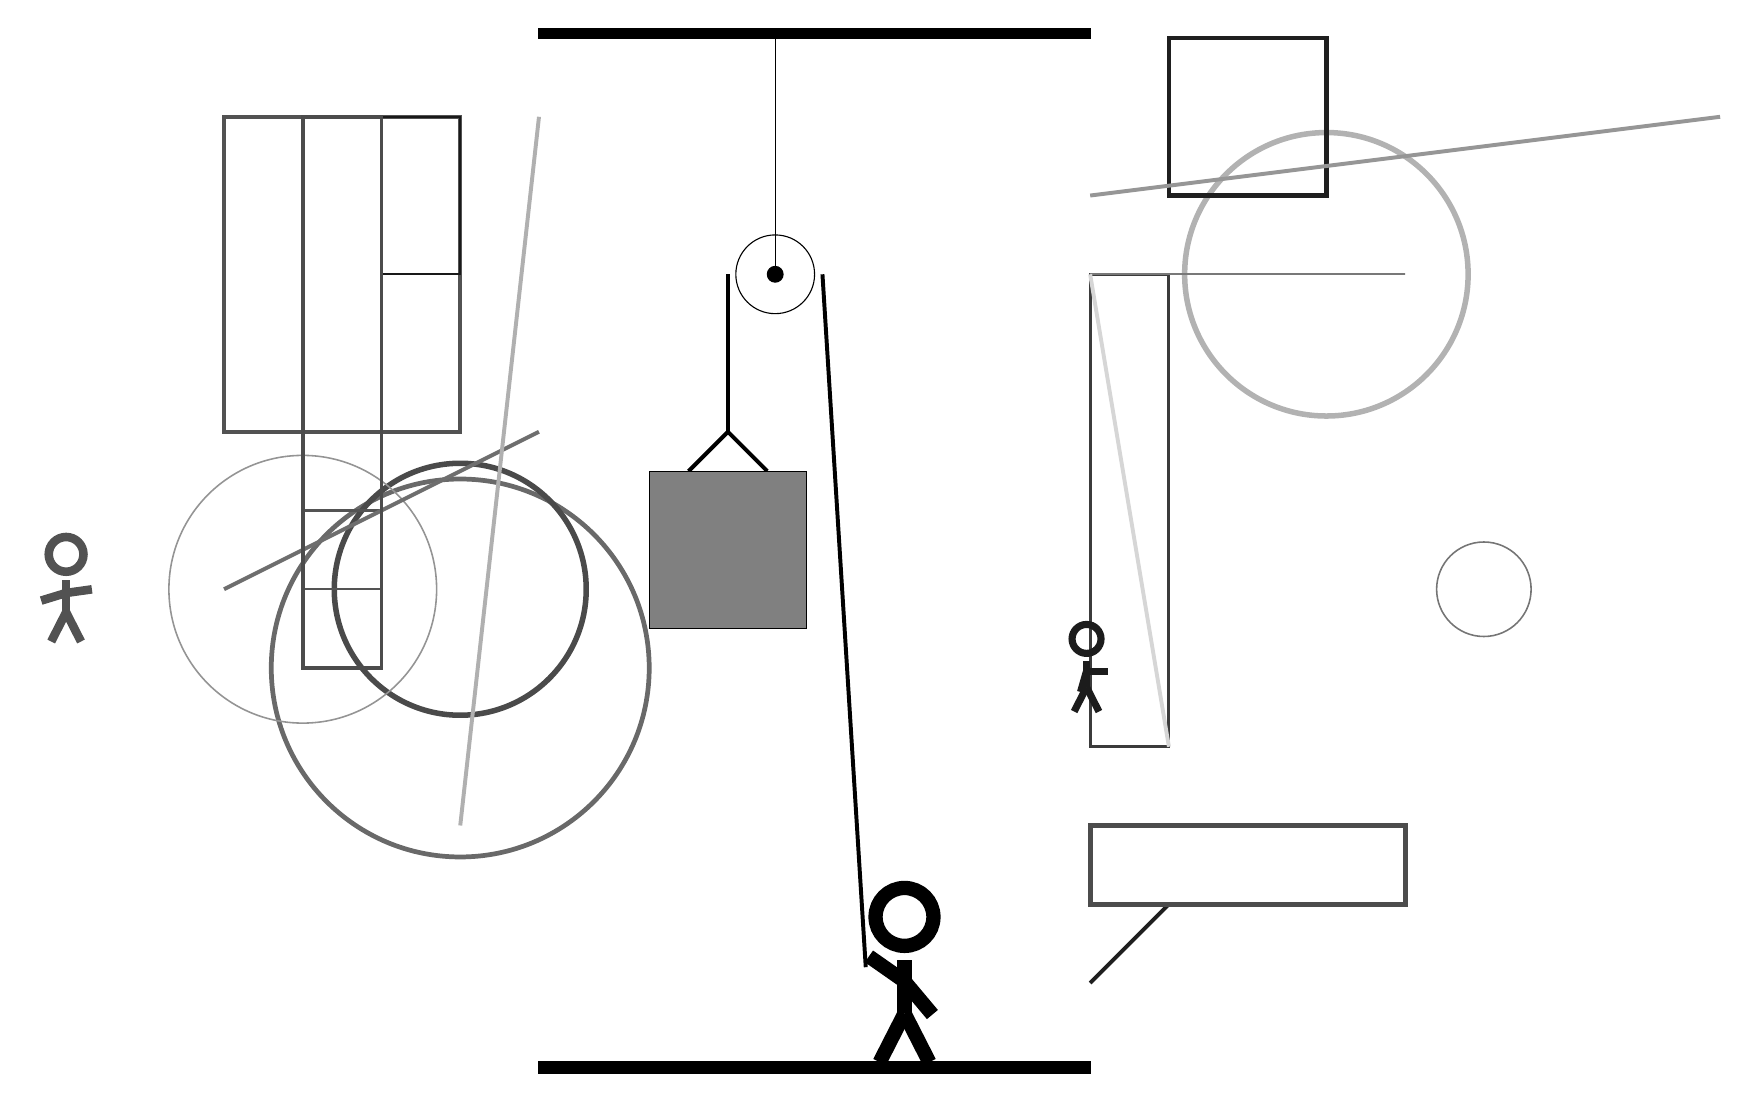
\begin{tikzpicture}
		%%%%% START %%%%%
		
		\draw[fill=black] (-2, 10) rectangle (5, 10.125);
		
		\draw [line width=0.6mm, color=black!59](-3, 2) circle (2.4);
		
		\draw [line width=0.7mm, color=black!71](-3, 3) circle (1.6);
		\draw[line width=0.4mm, color=black!77] (5, 1) rectangle (6, 7);
		\node[line width=0.3mm, color=black!68] at (-8, 3) {\Strichmaxerl[6][17][8]};
		\draw [line width=0.7mm, color=black!30](8, 7) circle (1.8);
		\draw[line width=0.2mm, color=black!53] (5, 7) rectangle (9, 7);
		\draw [line width=0.2mm, color=black!42](-5, 3) circle (1.7);
		
		\draw[line width=0.5mm, color=black!68] (-3, 5) rectangle (-6, 9);
		\draw[line width=0.3mm, color=black!90] (-4, 9) rectangle (-3, 7);
		
		\node[line width=0.2mm, color=black!89] at (5, 2) {\Strichmaxerl[5][74][0]};
		\draw[line width=0.3mm, color=black!67] (-4, 3) rectangle (-5, 4);
		
		\draw[line width=0.5mm, color=black!88](5, -2) -- (6, -1);
		\draw[line width=0.5mm, color=black!57](-6, 3) -- (-2, 5);
		
		\draw[line width=0.6mm, color=black!88] (6, 10) rectangle (8, 8);
		\draw[line width=0.6mm, color=black!70] (5, 0) rectangle (9, -1);
		\draw [line width=0.2mm, color=black!54](10, 3) circle (0.6);
		\draw[line width=0.5mm, color=black!41](5, 8) -- (13, 9);
		\draw[line width=0.5mm, color=black!31](-2, 9) -- (-3, 0);
		\draw[line width=0.5mm, color=black!70] (-4, 2) rectangle (-5, 9);
		
		\draw[line width=0.5mm, color=black!16](5, 7) -- (6, 1);
		
		\draw (1, 7) circle (0.5);
		\draw[fill=black] (1, 7) circle (0.1);
		\draw (1, 10) -- (1, 7);
		
		\draw[line width=0.5mm] (-0.1, 4.5) -- (0.4, 5.0) -- (0.9, 4.5);
		\draw[fill=black!50] (-0.6, 4.5) rectangle (1.4, 2.5);
		
		\draw[line width=0.5mm] (0.4, 7) -- (0.4, 5.0);
		\centerarc[line width=0.5mm](1, 7)(0:180:0.6);
		\draw[line width=0.5mm](1.6, 7) -- (2.15, -1.8);
		
		\node at (2.6, -1.9) {\Strichmaxerl[10][-35][-50]};
		
		\draw[fill=black] (-2, -3) rectangle (5, -3.15);
		
		%%%%% END %%%%%
	\end{tikzpicture}
\end{document}